%% abtex2-modelo-projeto-pesquisa.tex, v<VERSION> laurocesar
%% Copyright 2012-<COPYRIGHT_YEAR> by abnTeX2 group at http://www.abntex.net.br/
%%
%% This work may be distributed and/or modified under the
%% conditions of the LaTeX Project Public License, either version 1.3
%% of this license or (at your option) any later version.
%% The latest version of this license is in
%%   http://www.latex-project.org/lppl.txt
%% and version 1.3 or later is part of all distributions of LaTeX
%% version 2005/12/01 or later.
%%
%% This work has the LPPL maintenance status `maintained'.
%%
%% The Current Maintainer of this work is the abnTeX2 team, led
%% by Lauro César Araujo. Further information are available on
%% http://www.abntex.net.br/
%%
%% This work consists of the files abntex2-modelo-projeto-pesquisa.tex
%% and abntex2-modelo-references.bib
%%

% ------------------------------------------------------------------------
% ------------------------------------------------------------------------
% abnTeX2: Modelo de Projeto de pesquisa em conformidade com
% ABNT NBR 15287:2011 Informação e documentação - Projeto de pesquisa -
% Apresentação
% ------------------------------------------------------------------------
% ------------------------------------------------------------------------

\documentclass[
    % -- opções da classe memoir --
    12pt,                       % tamanho da fonte
    % openright,                % capítulos começam em pág ímpar (insere página vazia caso preciso)
    oneside,                    % para impressão em recto e verso. Oposto a oneside
    a4paper,                    % tamanho do papel.
    % -- opções da classe abntex2 --
    % chapter=TITLE,            % títulos de capítulos convertidos em letras maiúsculas
    % section=TITLE,            % títulos de seções convertidos em letras maiúsculas
    % subsection=TITLE,         % títulos de subseções convertidos em letras maiúsculas
    % subsubsection=TITLE,      % títulos de subsubseções convertidos em letras maiúsculas
    % -- opções do pacote babel --
    brazil,                     % idioma adicional para hifenização
    french,                     % idioma adicional para hifenização
    spanish,                    % idioma adicional para hifenização
    english,                    % o último idioma é o principal do documento
    ]{abntex2}

% ---
% PACOTES
% ---

% ---
% Pacotes fundamentais
% ---
\usepackage{lmodern}                                % Usa a fonte Latin Modern
\usepackage[T1]{fontenc}                            % Selecao de codigos de fonte.
\usepackage[utf8]{inputenc}                         % Codificacao do documento (conversão automática dos acentos)
\usepackage{indentfirst}                            % Indenta o primeiro parágrafo de cada seção.
\usepackage{color}                                  % Controle das cores
\usepackage{graphicx}                               % Inclusão de gráficos
\usepackage[babel=true, kerning=true]{microtype}    % para melhorias de justificação
% ---

% ---
% Pacotes adicionais
% ---
\usepackage{pdflscape}
\usepackage{adjustbox}
\usepackage{capa-epusp-abntex2}
\usepackage{pgfgantt} % gantt plot
\usepackage{rotating}
\usepackage[graphicx]{realboxes}
\usepackage{csquotes} % for babel
\usepackage{ragged2e} % provides \RaggedLeft
% ---

% ---
% Pacotes de citações
% ---
\usepackage[
    style=abnt,
    %style=authoryear,
    %citestyle=authoryear,
    %bibstyle=authortitle,
    %sorting=ynt,
    %backend=bibtex,
    %clearlang=true,
    %language=english,
    %natbib=true,
    %maxbibnames=99,
    %noslsn=true,
    %firstinits=true,
    %block=ragged,
    %ittitles,
    ]{biblatex} % Citações padrão ABNT
\addbibresource{biblio.bib}
% ---

% ---
% Informações de dados para CAPA e FOLHA DE ROSTO
% ---
\titulo{Increasing Power Efficiency on Convolutional Neural Networks for Field-Programmable Gate Arrays}
\autor{Vitor Finotti Ferreira}
\local{São Paulo}
\data{2017}
\instituicao{%
  Universidade de São Paulo
  \par
  Escola Politécnica
  \par
  Programa de Pós-Graduação - Engenharia de Computação e Sistemas Digitais}
\tipotrabalho{Master of Science Thesis}
\areaconcentracao{Computational Engineering}
% O preambulo deve conter o tipo do trabalho, o objetivo,
% o nome da instituição e a área de concentração
\preambulo{Proposal of a master thesis on the power efficiency improvement on convolutional neural networks in Field Programmable Gate Arrays.}
% ---

% informações do PDF
\makeatletter
\hypersetup{
    %pagebackref=true,
    pdftitle={\@title},
    pdfauthor={\@author},
    pdfsubject={\imprimirpreambulo},
    pdfcreator={LaTeX with abnTeX2},
    pdfkeywords={abnt}{latex}{abntex}{abntex2}{projeto de pesquisa},
    colorlinks=true,                    % false: boxed links; true: colored links
    linkcolor=blue,                     % color of internal links
    citecolor=blue,                     % color of links to bibliography
    filecolor=magenta,                  % color of file links
    urlcolor=blue,
    bookmarksdepth=4
}
\makeatother
% ---

% ---
% Espaçamentos entre linhas e parágrafos
% ---

% O tamanho do parágrafo é dado por:
\setlength{\parindent}{1.3cm}

% Controle do espaçamento entre um parágrafo e outro:
\setlength{\parskip}{0.2cm}  % tente também \onelineskip

% ---
% compila o indice
% ---
\makeindex
% ---

% ----
% Início do documento
% ----
\begin{document}

% Seleciona o idioma do documento (conforme pacotes do babel)
\selectlanguage{english}
%\selectlanguage{brazil}

% Retira espaço extra obsoleto entre as frases.
\frenchspacing

% ----------------------------------------------------------
% ELEMENTOS PRÉ-TEXTUAIS
% ----------------------------------------------------------
% \pretextual

% ---
% Capa
% ---
\imprimircapa
% ---

% ---
% Folha de rosto
% ---
\imprimirfolhaderosto
% ---

% ---
% NOTA DA ABNT NBR 15287:2011, p. 4:
%  ``Se exigido pela entidade, apresentar os dados curriculares do autor em
%     folha ou página distinta após a folha de rosto.''
% ---

% ---
% RESUMOS
% ---

% resumo em inglês
\begin{resumo}
     % Contextualization
     Convolutional neural networks have played a prominent role in recent years in the fields of computational vision, image recognition and machine learning.
     % Gap
     However, applications that require power efficiency are not favored by the use of the most commonly used hardware, the GPU, which delivers higher performance at the cost of higher power consumption when compared to other existing alternatives.
     % Objectives
     This project proposes to use techniques for optimization of hardware processing to improve the power efficiency of convolutional neural networks in FPGAs, which are attractive due to their greater flexibility and lower power consumption when compared to GPUs.
     % Methodology
     The topics to be explored in the search for a better power efficiency are sparsity of matrices, multiplications reduction and use of binary and ternary data types.

   \vspace{\onelineskip}
   \noindent
   \textbf{Keywords}: FPGA, Convolutional Neural Network, Power Efficiency.
\end{resumo}

% resumo em português
\setlength{\absparsep}{18pt} % ajusta o espaçamento dos parágrafos do resumo
\begin{resumo}[Resumo]
  \begin{otherlanguage*}{brazil}
    % Contextualization
    Redes neurais convolucionais têm tido um papel de destaque nos últimos anos nos campos de visão computacional, reconhecimento de imagens e aprendizado de máquina.
    % Gap
    Contudo, aplicações que necessitam de eficiência energética não são favorecidas pelo uso do hardware mais comumente usado, a GPU, que entrega maior desempenho ao custo de um maior consumo de energia se comparado a outras alternativas existentes.
    % Objectives
    Este projeto propõe aplicar técnicas atuais para otimização de processamento em hardware visando melhorar a eficiência energética de redes neurais convolucionais em FPGAs, hardware que possue o atrativo de maior flexibilidade e menor consumo energético que as GPUs.
    % Methodology
    Os tópicos a serem explorados na busca de uma melhor eficiência energética são a esparsidade de matrizes, a redução de multiplicações e o uso de formatos de dados binários e ternários.

 \textbf{Palavras-chave}: FPGA, Rede Neural Convolucional, Eficiência energética.
  \end{otherlanguage*}
\end{resumo}

% ---
% inserir o sumario
% ---
\pdfbookmark[0]{\contentsname}{toc}
\tableofcontents*
\cleardoublepage
% ---


% ----------------------------------------------------------
% ELEMENTOS TEXTUAIS
% ----------------------------------------------------------
\textual

% ----------------------------------------------------------
% Introdução
% ----------------------------------------------------------

\chapter[Introduction \& Background]{Introduction \& Background}
% Context (start introducing CNN)
%% say about CNN and FPGAs (GPUs are more powerful, but FPGAs are getting some space)
% Gap
%% Some applications require power efficiency due to energy limitations (Drones and autonomous systems)
%% GPUs have a bigger consumption than other platforms (e.g. FPGA)
%% necessidade de poupar energia onde der no robo, dado que não é possível fazer isso nos motores dado que eles oferecem pouca margem para otimizacoes energéticas dado sua natureza eletro-mecanica instrínseca
%% Introduce the project of the autonomous robot responsible for eliminating ipomoea vine on organic sugarcane plantations. (State the importance of agribusiness briefly also)
% Related work (State how the scientific community is tackling this issue)
%% Binary and Ternary data types
%% Pipeline
%% Pursued computational redundancy to reduce computational resources and energy consumption

Convolutional neural networks (CNNs) arouse as a leading solution in the field of computational vision, image recognition and machine learning in the last few years. The CNNs, although popular today, were overshadowed by other algorithms until the ImageNet competition in 2012, when their use almost halved the error rate of the other approaches~\cite{NIPS2012_4824}. This performance was only achieved by a combination of new training techniques and the efficient use of Graphics Processing Units (GPUs)~\cite{LeCun2015}.

Although GPUs are the paramount hardware for training neural networks due to its higher performance peak when compared to other architectures~\cite{Zhang2017, Nurvitadhi2017_1}, they also present higher power consumption~\cite{Sun2017}. In contexts where power availability is limited, such as drones and autonomous robots, the choice of hardware for image recognition has to be done carefully. High-performance hardware architectures can imply in a higher power consumption, reducing the autonomy of the robot, while more power-efficient solutions may result in slower processing, impacting the effectiveness of the recognition.

These challenges are suitable applications for Field-Programmable Gate Arrays (FPGAs), which have become an attractive solution to accelerate CNNs not only for its higher power efficiency, but also for its flexibility and short time-to-market~\cite{Zhang2017}. This has motivated efforts to optimize the power efficiency in this architecture while retaining recognition performance. A first topic of interest is exploring the FPGA parallelism, implementing a pipelined computational method for the processing in convolutional layers, which are computation-intensive as done by \textcite{Sun2017}. The high sparsity present in the neurons and weights of popular neural networks such as AlexNet, VGG and ResNet can be used, since sparse matrices require less multiplications than dense matrices~\cite{Nurvitadhi2017_1}. Fewer multiplications imply a lesser use of FPGA resources, resulting in lower power consumption. Another potential method to reduce multiplications is to reduce some redundant operations that happens on the convolutional layers, as suggested  by~\textcite{Ujiie2016}, so only the fundamental operations that affect the final result are executed. The use of binary and ternary data formats, instead of floating-point representation, is also a trend for increasing efficiency of CNNs due to the smaller memory space of the coefficients and the simpler arithmetic operations of these notations~\cite{Courbariaux2016c, NIPS2016_6573, Venkatesh2017}. The use of these compact data types introduces irregular parallelisms which are better mapped to FPGAs than GPUs~\cite{Nurvitadhi2017_1}.

% Estes esforços pela busca da eficiência de potência em CNNs e os consequentes benefícios que isto acarretaria para aplicações com recursos energéticos limitados ou com necessidade de eficiência energética inspirou este projeto, que tem como objetivo estudar de forma objetiva utilizar estas tendências na implementação energéticamente eficiente de redes neurais convolucionais em FPGAs.

These efforts to search for power efficiency in CNNs have inspired this project, which aims to analyse and use these trends in the pursue for a power efficient implementation of CNNs in FPGAs. This will be applied in the development of an image recognition system of an autonomous robot. This will be used in organic sugarcane farms to identify the \textit{Ipomoea grandifolia} vine, a weed present in these plantations, illustrated in \autoref{fig:ipomoea}. Such application is a

% Falar da importancia do agronegocio (o quanto ele representa do pib), o quanto a cana de acucar representa pro agro negocio (talvez falar em numeros), e citar que esforcos deste tipo tendem a permitir uso das tecnologias de CNN nao apenas neste setor, mas em diversas outras areas. Dizer que o estudo pode dar Maior independência dos dispositivos de reconhecimento de imagem (rede de internet movel, HW caro, alto consumo energético)

% Tal aplicação se mostra como uma das soluções mais víaveis para o problema, dado que o uso de herbicidas não é possível em plantações orgânicas, que o ambiente da hostil da plantação não favorece intervenção de trabalhadores humanos , e que processamento remoto das imagens obtidas é inviável por conta da comunicação sem fio precária por conta da humidade do ar intrínseca das plantações. Sendo assim, o reconhecimento de imagem tem de ser feito in loco, com o menor consumo enegético possível para aumentar a autonomia do sistema como um todo.

This application is shown as one of the most viable solutions to the problem, given that the use of herbicides is not possible in organic plantations, that the hostile environment of the plantation does not favor the intervention of human workers, and that remote processing of the images obtained is impracticable as a result of the poor wireless communication due the intrinsic air humidity of the plantations. Therefore, image recognition has to be done \textit{in loco}, with the lowest power consumption possible to increase the autonomy of the whole system.

\begin{figure}[htb]
  \caption{\label{fig:ipomoea}\textit{Ipomoea grandifolia} vine}
  \begin{center}
    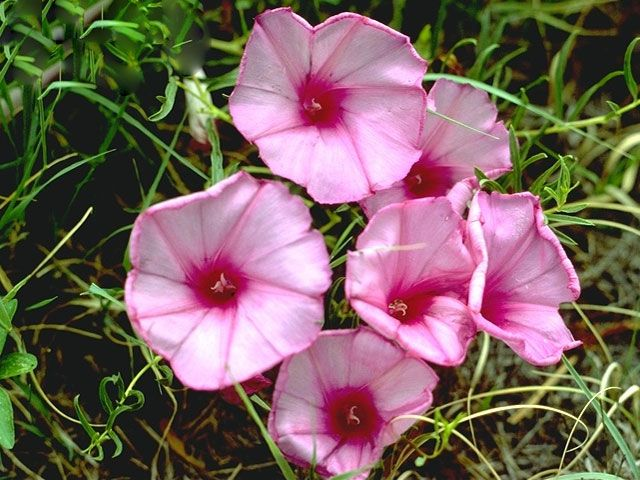
\includegraphics[scale=0.5]{images/Ipomoea_grandifolia76.jpg}
  \end{center}
  \legend{Source: \cite{corda_viola_agrolink}}
\end{figure}

%Introduce the area of research
%Review key publications
%Identify any gap in the knowledge or questions which have to be answered
%Your hypotheses
%Your aims and objectives, including a brief description of the methodology
%How is your research beneficial and to whom

\chapter[Objectives]{Objectives \& Motivation}

This work aims to obtain power efficiency in convolutional neural networks implemented in field-programmable gate arrays, while retaining image recognition capability for real time performance.

The acquired knowledge will be applied in the development of a image recognition system of the \textit{Ipomoea grandifolia}, a weed that affects sugarcane. Such identification would be the first stage of a system for the control of this pest.

The findings of this research could benefit applications with limited energy resources or in need of energy efficiency. This would bring more independence to image recognition devices, reducing the amount of resources needed to run these algorithms and allowing them to run on more economical and portable hardware.

\chapter[Methodology]{Methodology}
\section{Investigation Approach}

The first step towards the implementation is the study of the theory and background of neural network and image recognition for hardware accelerators. This will be done choosing appropriate disciplines simultaneously with the literature review so the most recent advances on the field can guide the theoretical development, as planned on \autoref{sec:scheadule}.

The knowledge obtained will be applied to develop the structure of a binary convolutional neural network to do the image recognition task. Recent studies, such as \textcite{Nurvitadhi2017_0} shows the potential of FPGAs in comparison with other architectures in terms of power efficiency. This potential is explored through specific optimizations on the neural network architecture, as mentioned on \textcites{Courbariaux2015, Zhang2017}. A training and test set of images of the \textit{Ipomoea grandifolia}, probably obtained from an organic sugarcane production farm, will be used to train the network and test its effectiveness in recognising the vine. This network will be trained using open-source tools.

Once the neural network is fully trained and tested, the implementation on hardware will begin. Tests to compare the performance and power consumption of the neural network on different architectures will be done, focusing in improving the power efficiency. The focus here is to reduce the power consumption to recognise one frame, while maintaining the frame rate suitable for real time performance of the system. The implemented network will be validated through simulations and empirical tests, using real or emulated data.

% Some studies suggest that FPGAs could outperform GPUs on next generations, using the combinations of numerous improvements made on FPGA together with DNN algorithm innovations that favour hardware customizability \cite{Nurvitadhi2017_1}. Achieving this performance on the FPGA could benefit not only this study, but also other applications that require not only energy efficience, but also high performance. Therefore, an effort will be made to improve the performance of the binary neural network as well.

\section{Tools and Resources}

  It is proposed to develop the project using open-source tools to reduce the cost of implementation and assist the dissemination of the technology created whenever possible. For the development phase, it will be used a computer with Linux operating system and software development environments such as Python and R. Since it is often necessary to use specific programs of the FPGA manufacturer for FPGA simulation, syntheses and implementation, private software such as Vivado or Quartus will be used. The infrastructure of the laboratories of the university will be used for the development and validation of the work done. Data for test and validation will be obtained from the an organic sugarcane production farm.

\section{Schedule} \label{sec:scheadule}
\begin{turn}{90}
  \begin{ganttchart}[vgrid={draw=none,draw=none},%
      % today=15,%
      % today offset=.5,%
      % today label=Heute,%
      % progress=today,%
      x unit=0.6cm,
      y unit title=0.7cm,
      y unit chart=0.55cm,
      bar incomplete/.append style={fill=red},%
      progress label text=  {\quad\pgfmathprintnumber[precision=0,verbatim]{#1}\%},%
      % progress label font=\tiny,
      % milestone label font=\tiny,
      % group label font=\tiny,
      % title label font=\tiny
      % bar label node/.style={text width=3cm,align=right,font=\scriptsize\RaggedLeft,anchor=east},
      % milestone label node/.style={text width=2cm,align=right,font=\scriptsize\RaggedLeft,anchor=east},
      % group label node/.style={text width=3cm,align=right,font=\scriptsize\RaggedLeft,anchor=east}
      ]{1}{24}
    \gantttitlecalendar*[compress calendar,time slot format=isodate]{2017-09-1}{2019-08-31}{year, month} \\
    \gantttitlelist{1,...,24}{1}\\
    \ganttgroup{Total Duration}{1}{24} \\
    %%%%%%%%%%%%%%%%% Disciplines
    \ganttgroup{Disciplines}{1}{16} \\
    \ganttbar{Discipline 1}{1}{4} \\
    \ganttbar{Discipline 2}{1}{4} \\
    \ganttlinkedbar{Discipline 3}{5}{9} \ganttnewline
    \ganttlinkedbar{Discipline 4}{10}{12} \ganttnewline
    \ganttlinkedbar{Discipline 5}{13}{16} \ganttnewline
    %%%%%%%%%%%%%%%%% Phase-1
    \ganttgroup{Phase 1}{1}{4} \\
    \ganttbar{Scope Reading}{1}{1} \\
    \ganttlinkedbar{Initial Literature Review}{2}{4} \ganttnewline
    %\ganttlinkedbar{Define Scope of Review}{3}{3} \ganttnewline
    %\ganttlinkedbar{Definition of Research Problem}{3}{3} \ganttnewline
    \ganttlinkedbar{Research Proposal Writing}{4}{4} \ganttnewline
    %%%%%%%%%%%%%%%%% Phase-2
    \ganttgroup{Phase 2}{5}{16} \\
    \ganttbar{Application Analysis}{5}{7} \\
    \ganttlinkedbar{Design Experimental Procedure}{7}{9} \ganttnewline
    \ganttlinkedbar{Development of source code}{8}{14} \ganttnewline
    \ganttlinkedbar{Run Experiments}{10}{16} \ganttnewline
    \ganttlinkedbar{Analysis of Experimental Data}{16}{19} \ganttnewline
    \ganttmilestone{Qualification Exam}{13} \\
    %%%%%%%%%%%%%%%%% Phase-3
    \ganttgroup{Phase 3}{17}{24} \\
    \ganttbar{Solving Validation and Conclusion}{17}{20} \\
    \ganttlinkedbar{Publications $\&$ Workshops}{19}{22} \ganttnewline
    \ganttlinkedbar{Thesis Writing}{19}{24} \ganttnewline
    \ganttmilestone{Thesis Defense}{23} \ganttnewline
    %%%%%%%%%%%%%%%%%%%%%%%%%%%%%%%%%%%%%%%%%%%%%%%%%%%%%%%%%%%%%%%
\end{ganttchart}
\end{turn}

\chapter{Expected Results}

%  Após a conclusão do projeto, é esperado que se tenha uma implementação de rede neural completamente funcional capaz de identificar o Ipomoea grandifolia em plantações de cana de açúcar com um mínimo de consumo energético. Espera-se também obter conhecimento das técnicas e medidas necessárias para implementar redes neurais em FPGAs de forma a otimizar seu o consumo energético e performance, tendo medidas quantitativas do resultado final. Comparações de eficiência energética e performance entre diferentes arquiteturas de hardware serão feitas, de forma que se possa avaliar as particularidades de cada uma e em quais situações a utilização de cada uma delas é mais propícia.

After conclusion of the project, it is expected to understand the techniques necessary to optimize power consumption of convolutional neural networks in FPGAs. Comparisons of power efficiency and performance obtained using different approaches, such as sparsity, multiplications reduction and use of binary and ternary data types will be made, so that one can evaluate the particularities of each one and their impact on the final system. Also, it is expected to have a fully functional neural network implementation capable of identifying \textit{Ipomoea grandifolia} vines in sugarcane plantations with a minimum of power consumption.


% ----------------------------------------------------------
% ELEMENTOS PÓS-TEXTUAIS
% ----------------------------------------------------------
\postextual

% ----------------------------------------------------------
% Referências bibliográficas
% ----------------------------------------------------------

\printbibliography

% ---

\end{document}

%%% Local Variables:
%%% mode: latex
%%% TeX-master: t
%%% End:
